\documentclass[11pt,a4paper]{article}

\usepackage[T1]{fontenc}
\usepackage[utf8]{inputenc}
\usepackage{lmodern}
\usepackage{amsmath,amssymb}
\usepackage{booktabs}
\usepackage{array}
\usepackage{longtable}
\usepackage{geometry}
\usepackage{xcolor}
\usepackage{graphicx}
\usepackage{hyperref}

\geometry{margin=1in}

\begin{document}

% ---------------------------------------------------------------- Week 2 (unchanged)
\section{Technical Analysis of BAKMM-IoD}
% Requires only: \usepackage{booktabs}
% All protocol identifiers are typeset using \texttt{} as requested.

\subsection{Technical Analysis of the BAKMM-IoD Protocol}
\label{subsec:technical-analysis-bakmm}

The BAKMM-IoD protocol consists of five major stages: registration, authentication
and key establishment, key management, dynamic device addition, and blockchain
formation. The registration and dynamic-device stages are trusted provisioning
operations, whereas the authentication and key-management stages are open-channel
cryptographic exchanges that can be represented directly in SPDL and verified using
Scyther. The paper explicitly describes the authentication phase as a three-message
exchange and the key-management phase as another three-message exchange. The
Scyther implementation uses \texttt{send}, \texttt{recv}, and the security claims
\texttt{Secret}, \texttt{Alive}, \texttt{Weakagree}, \texttt{Niagree}, and
\texttt{Nisynch}. The corrected SPDL models additionally represent the equality
checks in the protocol by using the expected cryptographic expressions directly as
receive patterns. This is important because an unconstrained declaration such as
\texttt{var m4} followed by \texttt{recv(...,m4,...)} does not model the protocol's
actual check \texttt{m4'}=\texttt{m4}.

\subsubsection{Registration and Credential Provisioning}

During registration, the trusted registration authority \texttt{RA} generates the
long-term credentials and derives pseudo-identities and temporal credentials. For a
drone \texttt{DEi}, the principal values are \texttt{RIDDEi} and \texttt{TCDEi};
for a ground station server \texttt{ESj}, they are \texttt{RIDESj} and
\texttt{TCESj}; and for a cloud server \texttt{CSk}, they are \texttt{RIDCSk} and
\texttt{TCCSk}. Each pseudo-identity requires one hash operation and each temporal
credential requires one additional hash operation. The common value
\texttt{RIDRA} is computed once as one hash operation. Consequently, the complete
registration of one \texttt{DEi}, one \texttt{ESj}, and one \texttt{CSk} requires
seven hash evaluations when \texttt{RIDRA} is included once:
three for \texttt{DEi}, two for \texttt{ESj}, and two for \texttt{CSk}.

Registration is not treated as an open-channel transaction in the SPDL model,
because the paper describes it as trusted provisioning and secure storage rather
than as an adversarial message exchange. Therefore its communication length is
not assigned a fabricated bit count. The corresponding SPDL file
\texttt{01\_registration.spdl} models the credential derivation computations only.

\begin{table}[ht]
\centering
\caption{Registration computation cost.}
\label{tab:bakmm-registration-cost}
\begin{tabular}{llll}
\toprule
Entity & Operation & Hash evaluations & Average server time \\
\midrule
\texttt{RA} & \texttt{RIDRA} & 1 & 0.055 ms \\
\texttt{DEi} provisioning & \texttt{RIDDEi}, \texttt{TCDEi} & 2 & 0.110 ms \\
\texttt{ESj} provisioning & \texttt{RIDESj}, \texttt{TCESj} & 2 & 0.110 ms \\
\texttt{CSk} provisioning & \texttt{RIDCSk}, \texttt{TCCSk} & 2 & 0.110 ms \\
\midrule
Total & & 7 & 0.385 ms \\
\bottomrule
\end{tabular}
\end{table}

The timing in Table~\ref{tab:bakmm-registration-cost} uses the average one-way
hash execution time \texttt{Th}=0.055 ms measured under the server platform
reported in the paper. The corresponding Raspberry Pi 3 average is
\texttt{Th}=0.309 ms.

\subsubsection{Authentication and Key Establishment}

The authentication phase establishes a common session key between \texttt{DEi} and
\texttt{ESj}. The three exchanged messages are

\begin{align}
\texttt{MSG1} &= \{\texttt{TIDDEi},\texttt{M1},\texttt{M2},\texttt{T1}\},\\
\texttt{MSG2} &= \{\texttt{M3},\texttt{M4},\texttt{M5},\texttt{T2}\},\\
\texttt{MSG3} &= \{\texttt{M6},\texttt{T3}\}.
\end{align}

The protocol uses fresh values \texttt{rs1}, \texttt{rs2}, \texttt{T1},
\texttt{T2}, and \texttt{T3}. The first message authenticates the drone through
\texttt{M2}. The second message provides the server contribution \texttt{rs2},
the session-key confirmation value \texttt{M4}, and the updated temporary
identity protected by \texttt{M5}. Finally, \texttt{M6} confirms to the ground
station server that the drone derived the same session key.

The session key is

\begin{equation}
\texttt{SKDEiESj} =
\texttt{h(h(TCDEi,rs1,MSDEiESj,T1),
h(RIDESj,TCESj,rs2,MSDEiESj,T2),
T1,T2,RIDDEi,MSDEiESj)}.
\end{equation}

For the communication-cost calculation, the paper assumes an identity and a
random number occupy 160 bits, an ECC point occupies 320 bits, a SHA-256 hash
occupies 256 bits, and a timestamp occupies 32 bits. Hence,

\begin{align}
L_{\texttt{MSG1}}
 &=160+256+256+32
 =704~\text{bits},\\
L_{\texttt{MSG2}}
 &=256+256+160+32
 =704~\text{bits},\\
L_{\texttt{MSG3}}
 &=256+32
 =288~\text{bits}.
\end{align}

Thus, direct calculation from the field sizes stated in the paper gives

\begin{equation}
L_{\mathrm{auth}}=704+704+288=1696~\text{bits}.
\end{equation}

The paper's comparative communication table reports a total of 1792 bits for
BAKMM-IoD. Therefore, there is a 96-bit discrepancy between the published total
and the direct calculation from the published field-size assumptions. The
reported value should not be silently substituted into the individual message
lengths; both values should be documented when reproducing the paper's analysis.

\begin{table}[ht]
\centering
\caption{Authentication message size and computation cost.}
\label{tab:bakmm-auth-cost}
\begin{tabular}{llllll}
\toprule
Message & Direction & Length & Sender hashes & Receiver hashes &
Purpose \\
\midrule
\texttt{MSG1} & \texttt{DEi}\rightarrow\texttt{ESj}
& 704 bits & 4 & 2 & Drone authentication \\
\texttt{MSG2} & \texttt{ESj}\rightarrow\texttt{DEi}
& 704 bits & 8 & 8 & Key establishment and server authentication \\
\texttt{MSG3} & \texttt{DEi}\rightarrow\texttt{ESj}
& 288 bits & 1 & 1 & Session-key confirmation \\
\midrule
Total & & 1696 bits & 13 & 11 & \\
\bottomrule
\end{tabular}
\end{table}

The sender-side hash counts are obtained directly from the equations. For
example, \texttt{DEi} evaluates two hashes for \texttt{M1}, two for
\texttt{M2}, three for the session key, and one for \texttt{M6}, giving
\texttt{8Th}. Similarly, \texttt{ESj} evaluates two hashes for \texttt{M3},
three for the session key, one for \texttt{M4}, and two for \texttt{M5}, also
giving \texttt{8Th}. This agrees with the paper's reported computation-cost
expression of approximately \texttt{8Th} per endpoint.

The receiver-side verification work is separate from the paper's simplified
\texttt{8Th} accounting. In particular, verification and recovery operations
introduce additional hash evaluations. Therefore, for a complete implementation
cost estimate, the verification computations should be included in addition to
the published sender-side estimate.

Using the paper's average execution times,
\texttt{Th}=0.055 ms on the server and \texttt{Th}=0.309 ms on Raspberry Pi 3,
the published \texttt{8Th} estimate corresponds to approximately
0.44 ms on the server and 2.47 ms on the Raspberry Pi 3.

\subsubsection{Key Management Between \texttt{ESj} and \texttt{CSk}}

The key-management phase follows the same three-message structure:

\begin{align}
\texttt{MSG1} &= \{\texttt{TINESj},\texttt{m1},\texttt{m2},\texttt{TS1}\},\\
\texttt{MSG2} &= \{\texttt{m3},\texttt{m4},\texttt{m5},\texttt{TS2}\},\\
\texttt{MSG3} &= \{\texttt{m6},\texttt{TS3}\}.
\end{align}

The session key is

\begin{equation}
\texttt{SKESjCSk} =
\texttt{h(h(RS2,TCCSk,MSESjCSk,TS2),
h(RS1,TCESj,MSESjCSk,TS1),
RIDESj,MSESjCSk,TS1,TS2)}.
\end{equation}

The message structure is analogous to the authentication phase. Under the same
field-size assumptions, the three messages have lengths

\begin{align}
L_{\texttt{MSG1}} &=160+256+256+32=704~\text{bits},\\
L_{\texttt{MSG2}} &=256+256+160+32=704~\text{bits},\\
L_{\texttt{MSG3}} &=256+32=288~\text{bits}.
\end{align}

Consequently, the calculated communication overhead is again

\begin{equation}
L_{\mathrm{KM}}=1696~\text{bits}.
\end{equation}

The paper does not provide a separate communication-cost entry for the
\texttt{ESj}-\texttt{CSk} key-management exchange; therefore this 1696-bit value
is a derived value based on the published field-size assumptions.

\begin{table}[ht]
\centering
\caption{Key-management message size and computation cost.}
\label{tab:bakmm-keymgmt-cost}
\begin{tabular}{llllll}
\toprule
Message & Direction & Length & Sender hashes & Receiver hashes &
Purpose \\
\midrule
\texttt{MSG1} & \texttt{ESj}\rightarrow\texttt{CSk}
& 704 bits & 4 & 2 & ES authentication \\
\texttt{MSG2} & \texttt{CSk}\rightarrow\texttt{ESj}
& 704 bits & 8 & 5 & Key establishment and confirmation \\
\texttt{MSG3} & \texttt{ESj}\rightarrow\texttt{CSk}
& 288 bits & 1 & 1 & Session-key confirmation \\
\midrule
Total & & 1696 bits & 13 & 8 & \\
\bottomrule
\end{tabular}
\end{table}

The sender-side generation cost is therefore \texttt{9Th} for \texttt{ESj} when
all its key-management values are generated, and \texttt{8Th} for \texttt{CSk}.
The additional receiver-side verification consists of two hashes for the
\texttt{MSG1} verification, five hashes for \texttt{MSG2} verification and one
hash for \texttt{MSG3} verification. Thus, the full symbolic computation count
is higher than the sender-only count. The sender-side total is
\texttt{17Th}, whereas including the receiver-side verification gives
\texttt{25Th}.

\subsubsection{Dynamic Device Addition}

The dynamic-device addition phase allows a new drone \texttt{DEv} to be added
without redesigning the complete network. The registration authority generates
\texttt{IDDEv}, \texttt{kDEv}, and \texttt{SNDEv}, then derives
\texttt{RIDDEv} and \texttt{TCDEv}. If \texttt{RIDRA} is already available, the
addition requires two new hash evaluations:

\begin{align}
\texttt{RIDDEv} &=
\texttt{h(RIDRA,IDDEv,kRA,kDEv,SNDEv)},\\
\texttt{TCDEv} &=
\texttt{h(RIDRA,IDDEv,kRA,kDEv,SNDEv,RTSDEv)}.
\end{align}

Hence the computational overhead is approximately \texttt{2Th}, corresponding
to 0.110 ms on the reported server platform or 0.618 ms on Raspberry Pi 3.
The paper describes the subsequent sharing of the registration information
with deployed ground-station servers as secure provisioning; since the exact
encoding of that provisioning message is not specified, its communication
length is not assigned an artificial bit count.

\subsubsection{Blockchain Formation}

After successful authentication and key management, \texttt{DEi} data are
received by \texttt{ESj}. The ground station creates transactions, encrypts
them using its ECC public key, constructs a partial block and sends the partial
block to a cloud server. The cloud server constructs the full block and
disseminates it through the peer-to-peer cloud-server network. A leader then
initiates pBFT consensus before the block is incorporated into the consortium
blockchain.

The transaction-level communication overhead is data-dependent. The paper
reports an additional 640 bits associated with the ECC representation of an
encrypted transaction, namely 320 bits for each of the two ECC point
components. Thus, for a plaintext transaction of length
\texttt{Ltrx}, the corresponding encrypted representation can be expressed as

\begin{equation}
L_{\texttt{encrypted\_trx}}
=
L_{\texttt{trx}}+640~\text{bits},
\end{equation}

subject to the exact ECC encoding used by the implementation.

The computation cost of the blockchain stage cannot be reduced to a single
hash count because it uses ECC encryption and ECDSA operations. The paper
reports average execution times of 0.674 ms and 2.288 ms for elliptic-curve
point multiplication on the server and Raspberry Pi 3, respectively, while
ECDSA generation averages 0.729 ms and 2.597 ms and ECDSA verification averages
1.405 ms and 4.901 ms on the two platforms. If one ECC point multiplication is
used as a coarse proxy for one ECC transaction-encryption operation, the
estimated encryption cost is approximately 0.674 ms on the server and
2.288 ms on Raspberry Pi 3. This is an approximation rather than a directly
reported encryption benchmark because the paper does not specify the exact
ECC encryption primitive or its complete operation count.

ECDSA signature generation and verification are block-level operations rather
than necessarily one operation per transaction. Therefore, their cost should
be multiplied by the number of blocks/signatures rather than by the number of
transactions unless the implementation explicitly signs each transaction.

\begin{table}[ht]
\centering
\caption{Blockchain computation primitives reported in the paper.}
\label{tab:bakmm-blockchain-cost}
\begin{tabular}{llll}
\toprule
Primitive & Symbol & Server average & Raspberry Pi 3 average \\
\midrule
Hash & \texttt{Th} & 0.055 ms & 0.309 ms \\
ECC point multiplication & \texttt{Tecm} & 0.674 ms & 2.288 ms \\
ECDSA generation & \texttt{Tecsigg} & 0.729 ms & 2.597 ms \\
ECDSA verification & \texttt{Tecsigv} & 1.405 ms & 4.901 ms \\
\bottomrule
\end{tabular}
\end{table}

\subsubsection{Overall Technical Assessment}

The corrected SPDL models preserve the central cryptographic structure of the
BAKMM-IoD protocol while correcting the most important modelling issue in the
initial implementation: received authentication values must be constrained by
their expected expressions. In the authentication phase, \texttt{M2},
\texttt{M4}, and \texttt{M6} therefore act as verification patterns rather than
unconstrained received variables. The same principle is applied to
\texttt{m2}, \texttt{m4}, and \texttt{m6} in the key-management phase.

The protocol has three principal security mechanisms. First, freshness is
provided by \texttt{T1}, \texttt{T2}, \texttt{T3}, \texttt{TS1}, \texttt{TS2},
and \texttt{TS3}. Second, authentication values are derived from secret
credentials, pseudo-identities, fresh random values and timestamps. Third, the
session keys combine long-term secrets with fresh session-specific values,
preventing an attacker from deriving a session key from public protocol
transcripts alone.

From a performance perspective, the cryptographic core is hash-dominated. The
paper therefore reports the authentication/key-establishment computation as
approximately \texttt{8Th} per endpoint, which corresponds to approximately
0.44 ms on the server and 2.47 ms on Raspberry Pi 3. The complete equation-level
analysis shows that receiver-side verification introduces additional hash
operations, so the published \texttt{8Th} value should be interpreted as a
simplified endpoint computation estimate rather than a complete accounting of
every verification operation.

The communication overhead of the three-message authentication exchange is
reported by the paper as 1792 bits, while direct recomputation using the paper's
own field sizes gives 1696 bits. This discrepancy should be explicitly recorded
in a technical report because reproducing the published total without
reconciling the individual field sizes would make the analysis internally
inconsistent.

Finally, the blockchain stage changes the dominant cost profile from lightweight
hashing to ECC and ECDSA operations. Consequently, the authentication and
key-management phases are computationally lightweight, whereas transaction
encryption and block-level signature processing constitute the comparatively
expensive operations. The practical blockchain experiment reported in the paper
also shows increasing computational time as the number of drones and ground
station servers increases, while the measured transaction throughput increases
across the evaluated deployment cases.


% ---------------------------------------------------------------- Week 3
\section{Week 3: Limitations, Research Gap and the Proposed FSL-AKE-IoD}
% Week 3: limitations of BAKMM-IoD, related work, research gap, FSL-AKE-IoD (v2), architecture,
% security and performance analysis.  Needs: booktabs, graphicx, amsmath, amssymb, longtable.
% Every number in this file is produced by proposed/code/*.py (see VERIFICATION_LOG.md).

\subsection{Limitations of BAKMM-IoD (verified)}
\label{subsec:w3-limitations}

All checks were run on a re-implementation of the drone ($DE_i$) to ground station ($ES_j$) phase
(\texttt{bakmm\_iod.py}) and on a literal transcription of the printed equations (\texttt{bakmm\_literal.py}).
The adversary is the paper's own: Dolev--Yao, CK, and physical drone capture with power analysis (\S3.2 of~[1]).
Table~\ref{tab:w3-flaws} summarises the verdicts.

\begin{table}[ht]
\centering
\caption{Claimed BAKMM-IoD flaws after independent verification.}
\label{tab:w3-flaws}
\small
\begin{tabular}{p{0.9cm}p{4.6cm}p{2.3cm}p{6.2cm}}
\toprule
Id & Flaw & Verdict & Evidence / condition \\
\midrule
A0 & Printed SK concatenation order differs between ES (AKDDE2) and DE (AKDDE3, Table 5) & CONFIRMED (erratum) & 0/1000 sessions agree with the printed formulas \\
A1 & Drone capture reveals all past and future SKs and links the TID chain & CONFIRMED & 5/5 past, 3/3 future SKs; contradicts Prop.~5, ASFF8, ASFF13, \S3.2 (forward secrecy). Not ASFF10. \\
A2 & Stolen ES table lets the adversary impersonate every drone; $TC_{DE}$ never checked & CONDITIONAL & needs read access to the ES database, which Prop.~4 assumes is prevented; the $TC_{DE}$ part is unconditional \\
A3 & One dropped message locks the drone out & CONFIRMED & both readings of the ES update (drop MSG3 / drop MSG2) \\
A4 & Replay of MSG1 inside $\Delta T$ & CONFIRMED / CONDITIONAL & accepted if the ES commits on MSG3; lock-out needs a single pending slot; rejected if the ES commits on MSG2 \\
A5 & \textbf{New:} M5 is not covered by M4; one flipped bit locks the drone out & CONFIRMED & both policies; contradicts Prop.~2 and ASFF2 \\
E & ES--CS phase as printed does not run & CONFIRMED & m1/m2 inner-hash order differ (CS m2 check fails); ES recovers $TIN^{new}$ with $RS_2$ it never learns \\
C & \S7.2 arithmetic & CONFIRMED & $704+800+288=1792$; the printed ``2880'' and ``1782'' are typos \\
\bottomrule
\end{tabular}
\end{table}

\paragraph{Why A1 is not caught by the paper's Scyther model.}
The paper's SPDL (Fig.~3/4) declares \texttt{const xor: Function}, an uninterpreted symbol without the cancellation
law. In such a model the intruder can never remove a mask $V\oplus h(RID_{DE}\|MS\|T)$, whatever it knows.
The ``no attacks within bounds'' result therefore says nothing about capture resistance.
The repository contains a capture model that encodes masking as encryption keyed by the mask
(\texttt{bakmm\_auth\_compromise.spdl}); its expected result is a failed SK secrecy claim.

\subsection{Comparison with related schemes}
\label{subsec:w3-related}

Security attributes are taken from Table~10 of~[1] (ASFF identifiers) unless marked ``unresolved''.
The source papers of~[2]--[4] are not in the repository, so the attributes that Table~10 does not cover
(forward secrecy, stolen verifier, de-synchronisation) could not be verified and are left as ``unresolved''.

\begin{table}[ht]
\centering
\caption{BAKMM-IoD, three related schemes and FSL-AKE-IoD (v2). Costs from Tables~8--9 of~[1]; ``*'' = broken in this work.}
\label{tab:w3-related}
\small
\begin{tabular}{p{3.0cm}p{2.1cm}p{2.1cm}p{2.1cm}p{2.1cm}p{2.3cm}}
\toprule
 & Bera et al.~[2] & Mishra et al.~[3] & Algarni \& Jan~[4] & BAKMM-IoD~[1] & FSL-AKE-IoD v2 \\
\midrule
Primitives & hash, ECC, AES & hash & hash (MD5), fuzzy extr. & hash, XOR & hash \\
Drone cost & $9T_h{+}2T_{senc}{+}2T_{ecm}{+}T_{eca}$ 7.405\,ms & $9T_h$ 2.78\,ms & $T_{fe}{+}14T_h$ 6.614\,ms & $8T_h$ 2.47\,ms & $5T_h$ 1.545\,ms \\
Server cost & 1.851\,ms & $7T_h$ 0.39\,ms & $6T_h$ \textbf{0.33\,ms} & $8T_h$ 0.44\,ms & $7T_h$ 0.385\,ms \\
Messages / bits & 3 / 2368 & 3 / 1792 & 4 / 2784 & 3 / 1792 & \textbf{2 / 1056} \\
Replay (ASFF1) & yes & yes & yes & no* (in $\Delta T$) & yes (cache to $T_1{+}\Delta T$) \\
Capture (ASFF8) & yes & yes & yes & no* & past: yes; KCI/future: no \\
Forward secrecy & unresolved & unresolved & unresolved & no* & drone side yes \\
Stolen verifier & unresolved & unresolved & unresolved & no* (if DB read) & yes (needs SE for $X_{ES}$) \\
De-sync resilience & unresolved & unresolved & unresolved & no* & yes (F3, F4) \\
Anonymity (ASFF13) & yes & yes & no & no* (after capture) & partial (retries linkable) \\
ESL (ASFF10) & yes & yes & no & yes & yes (vacuous: nonces public) \\
Dynamic addition (ASFF11) & yes & yes & no & yes & yes \\
Blockchain (ASFF12) & yes & no in~[1] Table~10 & no & yes & yes \\
Formal verification (ASFF9) & yes & yes & yes & $\times$ in Table~10 (Scyther in \S6) & models written, not run \\
\bottomrule
\end{tabular}
\end{table}

\subsection{Research gap}
\label{subsec:w3-gap}

\begin{enumerate}
\item \textbf{Forward secrecy at hash-only cost.} The hash-only IoD schemes derive every session key from static long-term
secrets (for BAKMM-IoD, verified: A1). ECC-based schemes can obtain forward secrecy but cost about $3\times$ more on the drone.
\item \textbf{Capture is argued, not modelled.} The published Scyther models omit key reveal and treat XOR as an uninterpreted function,
so capture attacks are invisible to them.
\item \textbf{State synchronisation.} Pseudonym rotation without a recovery path turns one lost or modified message into a permanent
lock-out (A3, A5).
\item \textbf{Edge verifier tables.} Ground stations are field-deployed yet store per-drone master keys in the clear (A2).
\item \textbf{Cost.} Among the compared schemes, FSL-AKE-IoD v2 is the cheapest on the drone and in communication,
but not on the server (Algarni \& Jan: $6T_h$).
\end{enumerate}

\subsection{Proposed protocol: FSL-AKE-IoD (v2)}
\label{subsec:w3-protocol}

$DE_i$ stores $\{TID_i,K_i\}$. $ES_j$ keeps $X_{ES}$ in a secure element and stores masked records
$C_i=K_i\oplus h(X_{ES}\|TID_i)$.
\begin{align}
MSG_1 &= \{TID,N_1,T_1,V_1\}, & V_1 &= h(K\|TID\|N_1\|T_1) & (608~\text{bits})\\
SK &= h(K\|N_1\|N_2\|T_1\|T_2\|TID), & & & \\
MSG_2 &= \{N_2,T_2,V_2\}, & V_2 &= h(SK\|N_2\|T_2) & (448~\text{bits})\\
K &\leftarrow h(K\|SK), & TID &\leftarrow h(TID\|SK)_{[0..159]} &
\end{align}
The review of the draft version (v1) found four flaws and fixed them:
\textbf{F1}, a unique device id per drone (v1's default id made one drone's session delete every other drone);
\textbf{F2}, replay-cache entries kept until $T_1+\Delta T$ rather than receive time $+\Delta T$ (otherwise a replay
under legal clock skew is accepted and locks the drone out);
\textbf{F3}, the ES keeps the last proven key as the \emph{anchor} plus every \emph{candidate} derived from it, and
promotes a candidate only when the drone proves it holds it (v1's single old/current pair is broken by a reordered
retry);
\textbf{F4}, the drone waits more than $2\Delta T$ before re-sending on the same credentials, so the bounded candidate
list cannot be evicted.
In addition, the ES refuses $MSG_1$ for $2\Delta T$ after a reboot, tries every record stored under a TID
(collision tolerance), and revocation deletes the anchor and all candidates. The ES--CS key management uses the same
exchange with $ES_j$ as initiator.

\subsection{Architecture}
\label{subsec:w3-arch}

The architecture has four layers: drones (5 hash operations per session); ground stations (secure element, masked
anchor and candidate records, replay cache, ECC/ECDSA partial blocks); cloud servers (P2P, pBFT); and the offline RA,
which must erase $K_i$ after provisioning. Figure sources are \texttt{fslake\_architecture.dot} and
\texttt{fslake\_auth.dot}; the SVGs are in the repository root.

\subsection{Security analysis}
\label{subsec:w3-security}

32 attacks were run against BAKMM-IoD (both ES update policies), the draft protocol (v1) and v2
(\texttt{attacks\_fslake.py}, reproduced by \texttt{tests/test\_protocols.py}). Nine attacks succeed against v1:
replay under clock skew, replay after an ES reboot, a reordered retry, withheld-retry eviction, a second drone's
record being deleted, naive revocation, TID-collision overwrite, and the two inherent ones below. v2 resists all of
these. The limitations that remain for v2 are inherent to a symmetric-key-only design, or are partial:
\begin{itemize}
\item KCI after drone capture, and future sessions after capture (no post-compromise security);
\item full ES compromise with $X_{ES}$ exposes the last session of each drone (3/15 in the experiment) and all future ones;
      adding a key-confirmation $MSG_3$ lowers this to 0/15 without ECDH;
\item failed attempts reuse the TID, so an active adversary that drops MSG2 can track a drone (optional retry pseudonyms remove this at $+w$ ES hashes);
\item an RA that keeps $K_0$ and records every transcript learns every SK (the chain breaks after one missed transcript);
\item clock drift beyond $\Delta T$ and roaming across ground stations with one credential.
\end{itemize}
The ablation (\texttt{ablation.py}) shows that each of M1--M5 and F2--F4 is necessary: switching one off re-opens a
specific attack. M6 (two messages) re-opens nothing; it is a cost optimisation that gives up ES-side forward secrecy
of the last session.
A Real-or-Random proof sketch is in \texttt{FSL-AKE-IoD-security\_verification.ipynb}; its bound is
$\mathrm{Adv}\le q_h^2/2^{256}+(q_s+q_e)^2/2^{160}+(2q_s+2q_h)/2^{256}$.
Scyther and ProVerif models (plain, capture, and a control model) were written but \textbf{not run}, because
neither tool is installed on the authoring machine.

\subsection{Performance analysis}
\label{subsec:w3-performance}

Hash counts were obtained by instrumenting $h(\cdot)$: BAKMM-IoD takes 8 on the drone (3+5) and 8 on the ES (7+1);
FSL-AKE-IoD v1 and v2 both take 5 and 7. With the paper's $T_h$ (0.309\,ms Raspberry Pi~3, 0.055\,ms server), the drone
cost falls from 2.472 to 1.545\,ms ($-37.5\%$), the server cost from 0.440 to 0.385\,ms ($-12.5\%$), and
communication from 1792 to 1056 bits ($-41.1\%$, 3$\to$2 messages).
FSL-AKE-IoD v2 has the lowest drone cost and the lowest communication of all compared schemes. On the server it is
\textbf{not} the cheapest: Algarni \& Jan need $6T_h$ (0.33\,ms), and Mishra et al.\ equal it at $7T_h$.
On the authoring PC one SHA-256 call through $h(\cdot)$ took about $7\,\mu$s on average ($10^5$ runs), and a full
FSL-AKE-IoD session took less time than a BAKMM-IoD session.

\begin{figure}[ht]
\centering
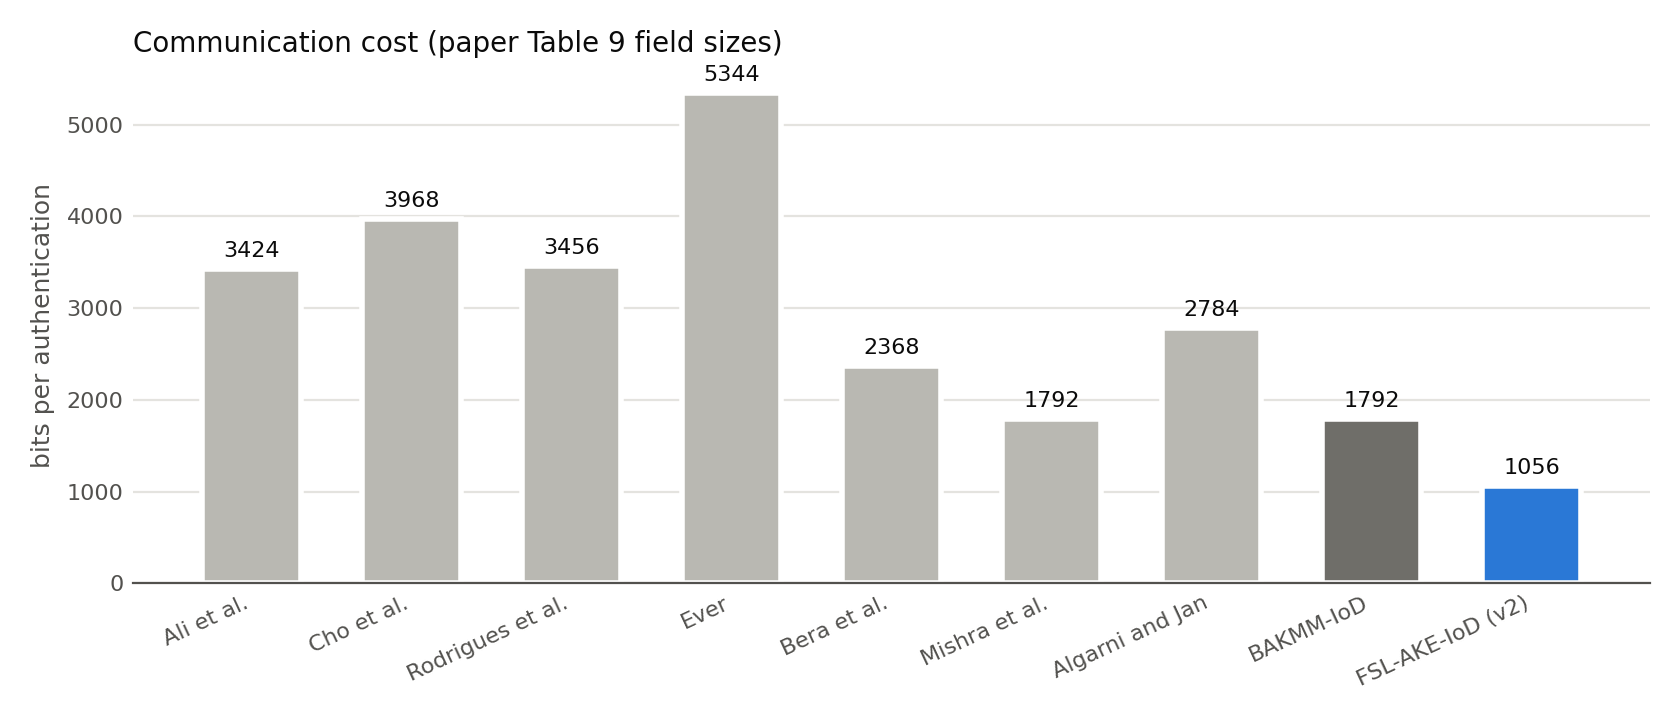
\includegraphics[width=0.48\textwidth]{images/fslake_comm_cost.png}\hfill
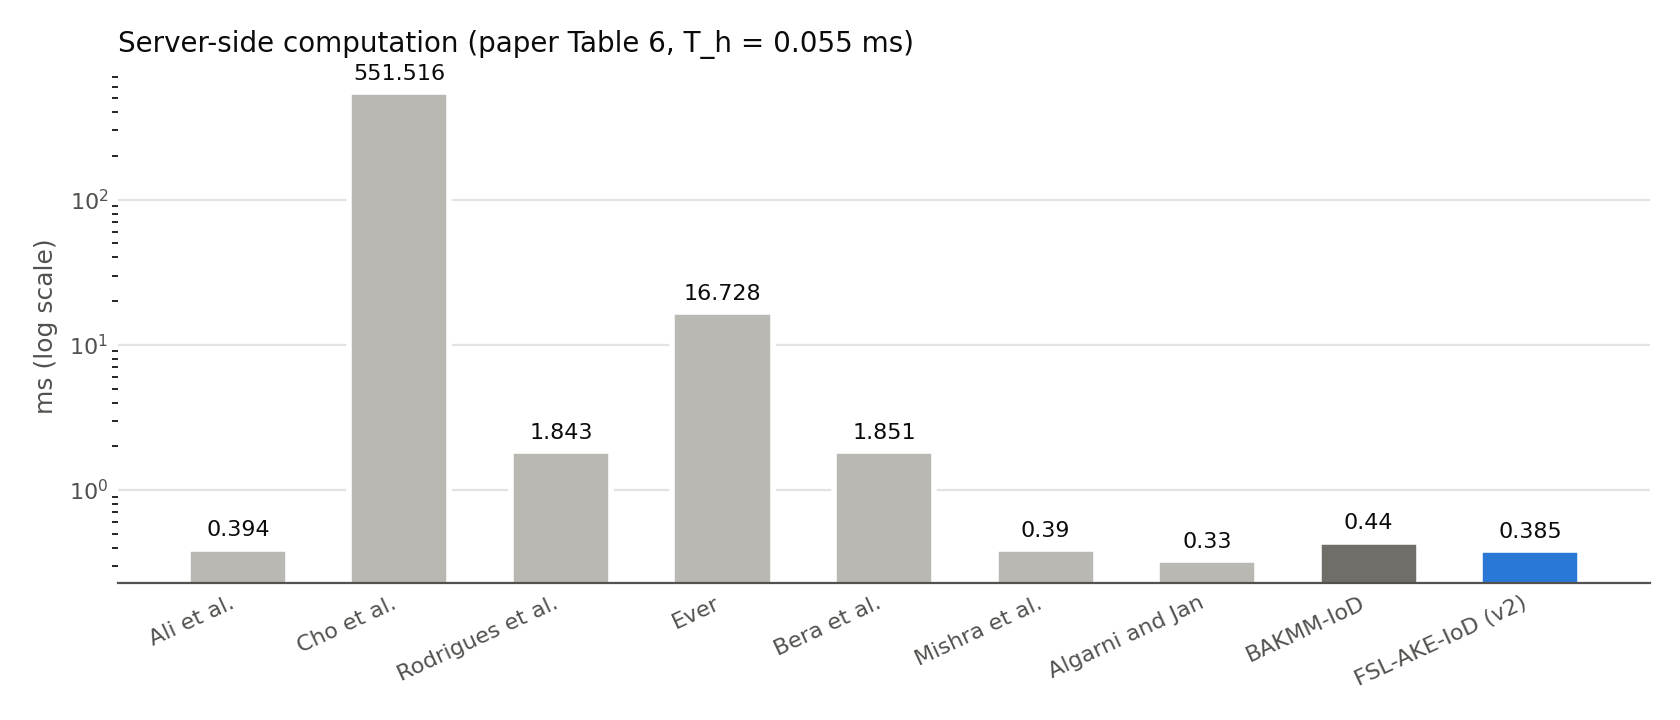
\includegraphics[width=0.48\textwidth]{images/fslake_server_cost.png}
\caption{Communication cost and server-side computation (Tables~8--9 of~[1] plus FSL-AKE-IoD v2).}
\label{fig:w3-cost}
\end{figure}


\subsection*{References}
\begin{enumerate}
\item[{[1]}] M. Wazid, S. Mittal, A. K. Das, SK H. Islam, M. J. F. Alenazi, A. V. Vasilakos, ``Designing secure
blockchain-based authentication and key management mechanism for Internet of Drones applications,''
J. Syst. Archit. 160 (2025) 103365.
\item[{[2]}] B. Bera, A. K. Das, A. K. Sutrala, ``Private blockchain-based access control mechanism for unauthorized UAV
detection and mitigation in Internet of Drones environment,'' Comput. Commun. 166 (2021) 91--109.
\item[{[3]}] A. K. Mishra, M. Wazid, D. P. Singh, A. K. Das, J. Singh, A. V. Vasilakos, ``Secure blockchain-enabled
authentication key management framework with big data analytics for drones in networks beyond 5G applications,''
Drones 7(8) (2023).
\item[{[4]}] F. Algarni, S. U. Jan, ``PSLAPS-IoD: A provable secure and lightweight authentication protocol for securing
Internet-of-Drones (IoD) environment,'' IEEE Access 12 (2024) 45948--45960.
\end{enumerate}

\end{document}
